\subsection{CAESSC}
%TODO: rewrite 
The model is the following:
\begin{figure}[H]
    \centering
    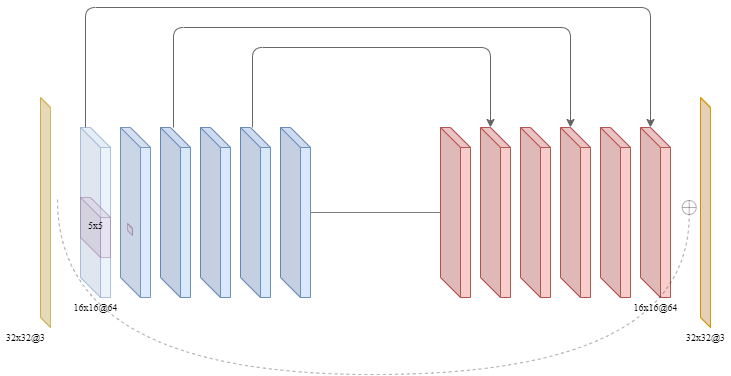
\includegraphics[scale=0.4]{subsections/caessc/caessc.png}
\end{figure}

In order to achieve good result for low-level image processing as deblurring, super-resolution, deep network are necessary.
Nevertheless the deeper the network the slower the training is thus skip connections are used between symmetric convolutional and deconvolutional layers.

Features are extracted by convolutional layers (encoder) and information are used by deconvolutional layer (decoder) for reconstructing the image; moreover symmetric  skip connections are used for increasing performance and the ability to converge of the network.

The architecture is quite simple:
\begin{itemize}
    \item The downsampling is done by a \textit{Conv2D} layer at the beginning.
    The researchers observed that an earlier downsampling allow to decrease the testing time with a small reduction of the performance.
    \item Encoder-Decoder architecture where convolutional and deconvolutional layers are connected symmetrically
    \item A skip connection between the input and the output allow to learn the output deblurred without the skip connection plus all the details learned by the encoder. \footnote{Refer to \cite[4.1 Analysis of the architecture]{CAESSC}} 
\end{itemize}

Skip connections have important goals \cite{resnet}:
\begin{enumerate}
    \item Networks are easy to optimize using the identity function
    \item The features information are forwarded from convolutional to deconvolutional layer facilitating the work of deconvolutional layer for reconstructing the image increasing the performance of the network.
    \item Overcame \textbf{vanishing gradient}: the weights are not updated when the network is deeper because gradients became smaller and smaller the deeper the network is.
    \item Overcame \textbf{exploding gradient}: the backpropagation of the gradient could lead to an exponentially increase of the gradient the deeper the network is.
\end{enumerate}

The model implemented were two:
\newcommandx{\CAESSC}[3][3={}]{CAESSC\_d{#1}\_f{#2}{#3}}

\begin{itemize}
    \item \CAESSC{30}{64}: depth equals to 30, filters equal to 64 and no downsampling applied.
    \item \CAESSC{22}{128}{half}: depth equals to 22, filters equal to 128 and downsampling applied.
\end{itemize}

\subsection{Training}
The network was trained using Adam\cite{adam} with $1e^{-4}$ as learning rate, MSE as loss function and with an early stopping equals to 7 in order to push more the training.

\subsection{Results}
\CAESSC{30}{64}, . converged, respectively, after . and . epochs with early stopping equals to 6.

\begin{figure}[H]
    \begin{subfigure}{\textwidth}
        \centering
        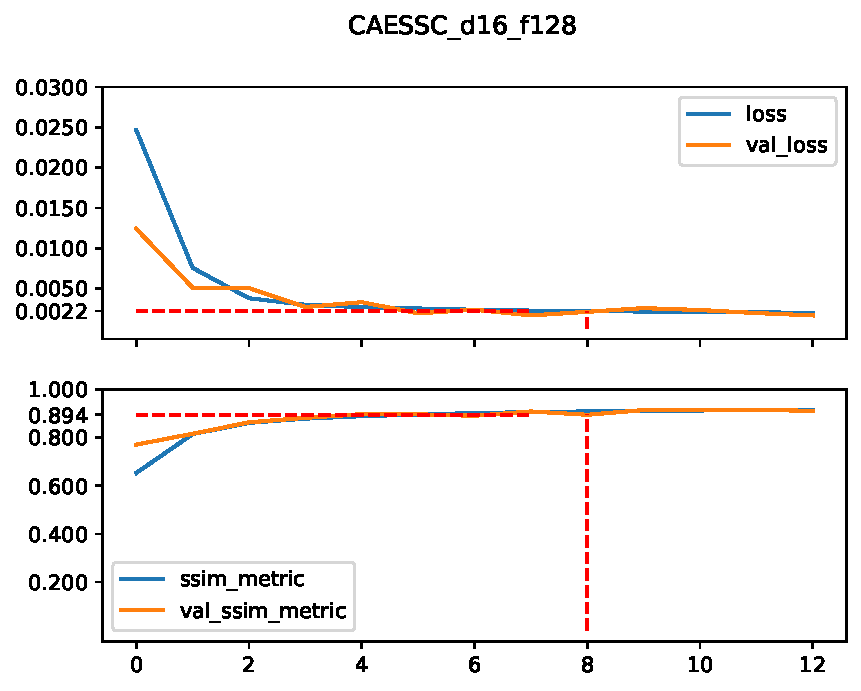
\includegraphics[height=0.37\textheight,keepaspectratio]{subsections/caessc/plot_history_CAESSC_d16_f128.pdf}
    \end{subfigure}
    \begin{subfigure}{\textwidth}
        \centering
        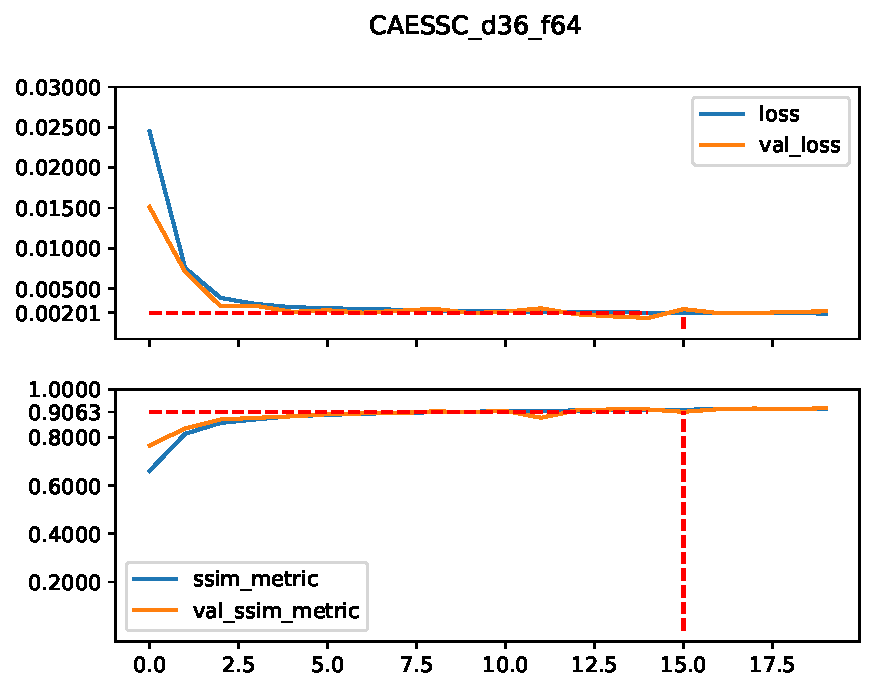
\includegraphics[height=0.37\textheight,keepaspectratio]{subsections/caessc/plot_history_CAESSC_d36_f64.pdf}
    \end{subfigure}
\end{figure} 

The evaluation of the networks is the following:

\begin{tabularx}{300pt}{ccccc}
    & \multicolumn{3}{c}{CAESSC} & {RED30} \footnote{RED30 is composed by 30 layers with skip connections every 2 layers, 128 filters and kernel size equal to 3. Taken from \url{https://github.com/ved27/RED-net/blob/master/model/REDNet_ch3.prototxt and /model/debluring/gaussian.caffemodel}} \\
    network & MSE & PSNR & SSIM & PSNR  \\
    CAESSC\_d16\_f128 & 0.0019 & 28.56 & 0.91 & 34.49 \\
    CAESSC\_d32\_f64 & 0.0017 & 29.00 & 0.92 & 34.49
\end{tabularx}


\begin{figure}[H]
    \centering
    \begin{subfigure}{\textwidth}
        \centering
        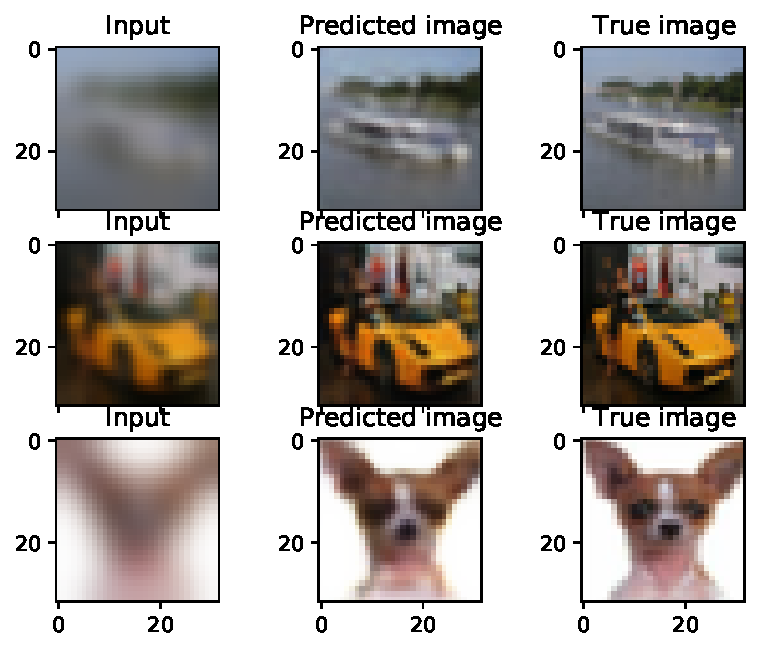
\includegraphics[height=0.35\textheight,keepaspectratio]{subsections/caessc/d16_f128.pdf}
        \caption{Network CAESSC\_d16\_f128}    
    \end{subfigure}
    \begin{subfigure}{\textwidth}
        \centering
        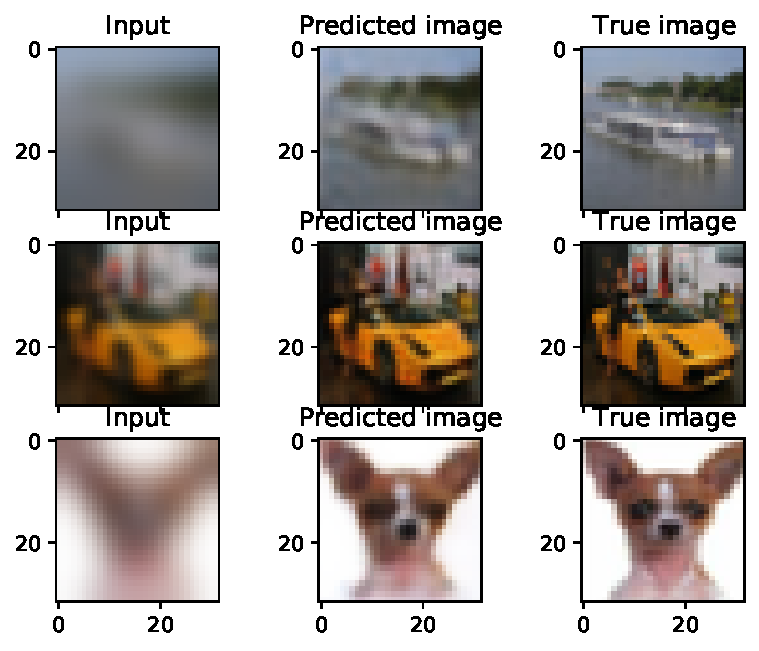
\includegraphics[height=0.35\textheight,keepaspectratio]{subsections/caessc/d36_f64.pdf}
        \caption{Network CAESSC\_d32\_f64}            
    \end{subfigure}
    
    \caption{Test image generated by CAESSC.}
\end{figure}

